\documentclass[a4paper,11pt]{article}
\usepackage[utf8]{inputenc} %pour utiliser tous les caracteres du clavier 
\usepackage[T1]{fontenc} %meme chose ici
\usepackage[francais]{babel} %pour ecrire en francais
\usepackage{listings} %pour citer du code

\usepackage{amsfonts} % pour utiliser les symboles de ensembles (reel...autre)
\usepackage{amsmath} %debut des package pour utiliser les formules de math
\usepackage{amssymb}
\usepackage{mathrsfs}
\usepackage[top=2cm, bottom=2cm, left=2.0cm, right=1.9cm]{geometry}

\usepackage{graphicx} %pour charger des images
\usepackage{float}

\usepackage{textcomp}
\lstset{
%upquote=true,
columns=flexible,
basicstyle=\ttfamily,}

\title{Application Android: Arboretum\\
Rapport}
\author{Barbier Jérôme, Benyounes Radhoane, Bobo William\\ Fréby Rodolphe, Husson Augustin, Labat Paul}
\date{\today}

\begin{document}
   \maketitle

  \begin{center}
    
\includegraphics{logoPol.jpg}\\
    %Rapport généré avec \LaTeX
  \end{center}
  \tableofcontents
  \newpage
  
  \section{Introduction}
    \subsection{But de ce Rapport}
  Ce rapport a été rédigé pour nous permettre d'expliquer en détail nos choix de conception. Il permettra également en cas de reprise de ce projet 
  d'avoir une connaissance approfondie de l'ensemble des fonctionnalités qui a été implémenté.
  
    \subsection{Présentation du Projet}
    Le projet s'intitule \textit{Arboretum}. Il s'agit de faire une application qui permettra à l'utilisateur de faire une visite guidée du parc.
    Ce parc se situe à l'extrémité Nord Est du campus de Grenoble en France. L'application doit permettre à l'utilisateur de se rendre dans le parc
    et de faire la visite guidée. Elle doit également lui permettre de faire la visite sans y être. 
    
    La particularité de ce parc est qu'il y a une représentation à échelle réduite de notre Galaxie. On y trouve également des espèces d'arbres et de plantes
    peu communes. L'application doit permettre de naviguer entre les arbres et les planètes et de fournir une description détaillée pour chacun d'entre eux.
    \subsection{Spécification technique}
      \begin{itemize}
       \item Configuration nécessaire : Android 4.1
       \item Un capteur NFC est nécessaire pour profiter de toutes les fonctionnalités de l'application
       \item Place prise sur le stockage interne : 14,42Mo pour l'application, et 3,5Mo de données téléchargées.
       \item L'application requiert une autorisation d'utiliser : 
     \begin{itemize}
      \item le stockage
      \item votre position (via le GPS)
      \item la communication réseau (c'est à dire avoir un accès Internet complet, ainsi qu'avoir le contrôle NFC)
      \item les commandes matérielles (c'est-à-dire prendre des photos et des vidéos)
     \end{itemize}
      \end{itemize}

   \section{Architecture}
    \begin{figure}[H]
     \begin{center}
      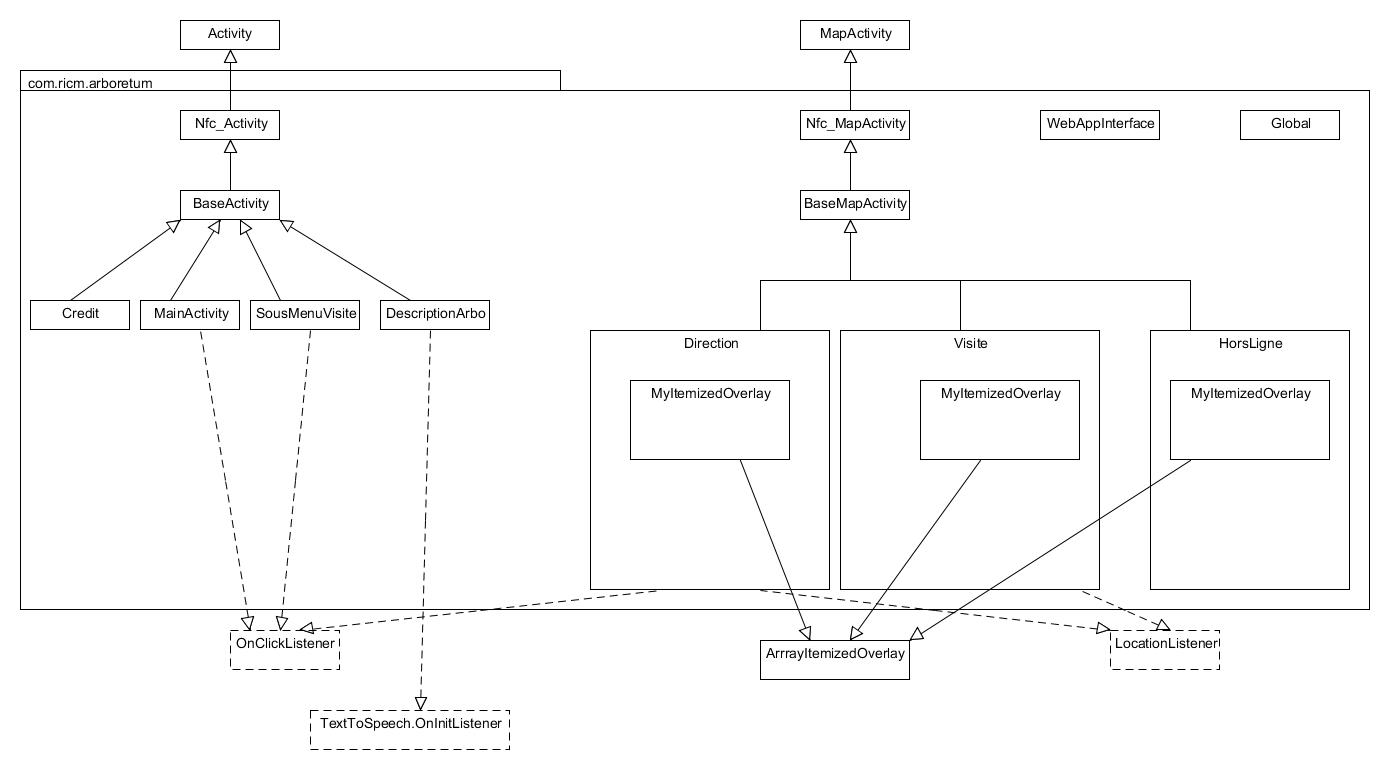
\includegraphics[width=18cm,height=10cm]{archi.jpg}
      \caption{Architecture globale}
     \end{center}
    \end{figure}
    Comme on peut le voir, nous avons un package principal com.ricm.arboretum. Dans ce package on trouve deux arbres d'héritage principaux. Le premier 
    ayant pour classe mère Activity, et l'autre ayant pour classe mère MapActivity.
    
    Le premier arbre est l'implémentation des activités générales qui composent l'application et le second est l'implémentation de toutes les activités 
    qui nécessitent la présence d'une map.
    
    On remarque que certaines classes sont en dehors du package. La différence est faite si la classe a été conçue par notre équipe ou fournit par des packages externes.
      \newpage
		\section{Gestion des menus}
		
		L'application met à disposition un système de différentes \emph{activités} pour pouvoir accéder aux fonctionnalités désirées. 
		L'utilisateur arrive sur un menu principal lui demandant s'il souhaite se rendre à l'arboretum ou visiter celui-ci. 
    \begin{figure}[H]
     \begin{center}
      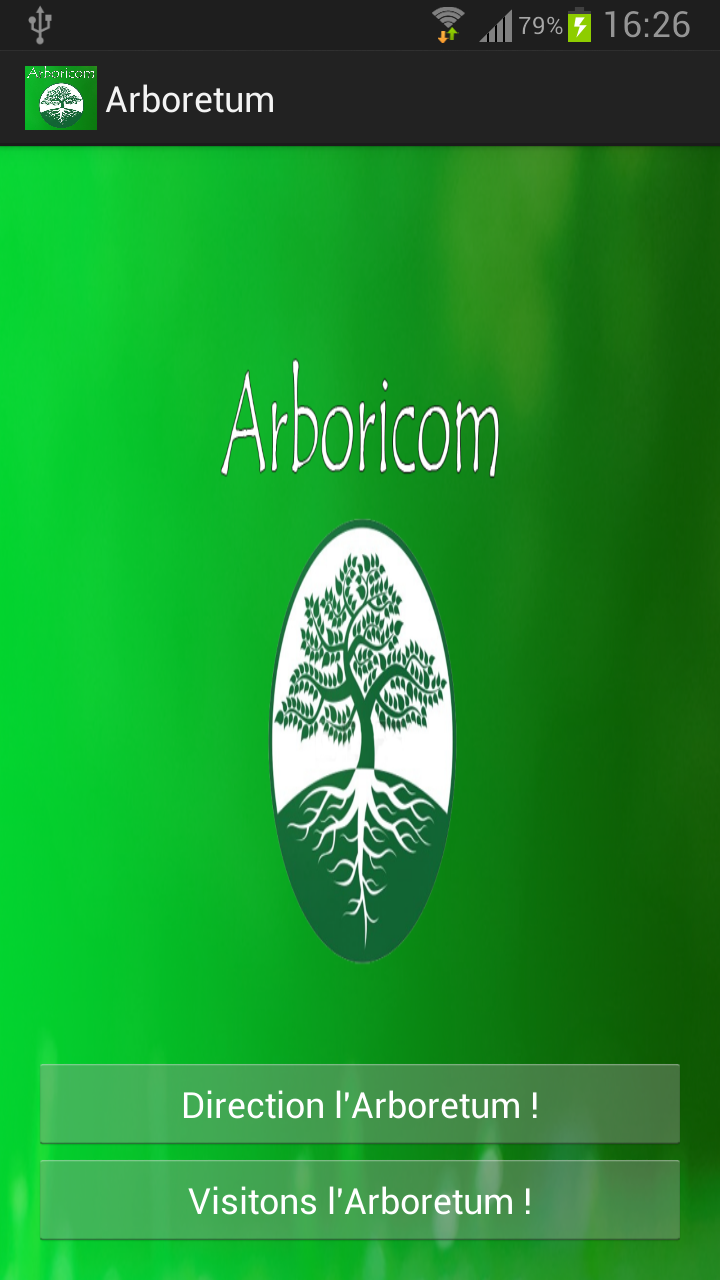
\includegraphics[width=5cm,height=8cm]{menu.png}
      \caption{Menu Principal sur un \textit{Samsung Galaxy S3}}
     \end{center}
    \end{figure}
		Dans le deuxième cas, il peut choisir entre une visite dite ``en ligne'' utilisant les services de localisation, ou ``hors ligne''. 
		Au travers de la totalité des classes, par héritage avec \emph{BaseActivity} ou \emph{BaseMapActivity}, l'utilisateur possède un accès 
		à un sous-menu paramètre, permettant d'activer ou non le son, de prendre des photos, ou bien d’accéder au crédit. 
		Il est important de noter que les crédits sont constamment accessibles sauf lorsque l'utilisateur visionne ceux-ci. 
    \begin{figure}[H]
     \begin{center}
      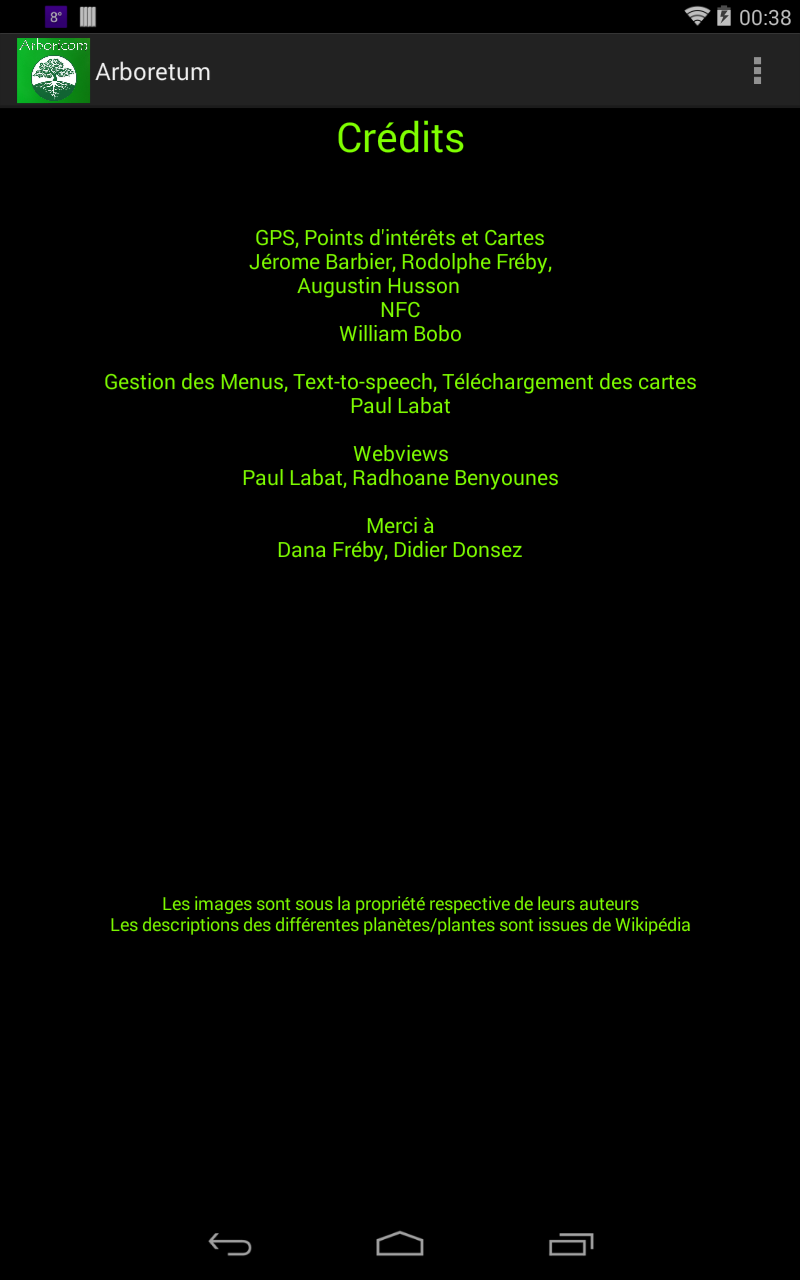
\includegraphics[width=7cm,height=9cm]{credit.png}
      \caption{Page des Crédits}
     \end{center}
    \end{figure}
		La gestion du son est global, ainsi la désactivation de celui-ci (qui désactive le son des notifications lors de la visite en ligne) est prise en compte sur la totalité de l'application. 
		Un autre point important réside dans le fait que bloquer le son ne bloque pas les notifications sonores de manière définitive. En effet, si un utilisateur désactive puis réactive le son, 
		les objets devant lesquels il était déjà passé ne seront pas comptés comme ayant été dépassé, et peuvent ainsi émettre un son lors d'un passage de l'utilisateur devant le point d’intérêt en question. 
		Il s'agit là d'un choix d'implémentation de notre part.
		Les photos prisent avec l'appareil possède un nommage numérique incrémentée automatiquement, et sont stockées dans \emph{/arboretum/photos/}. 
		Une autre particularité de notre application est la création des différents répertoires nécessaires au bon fonctionnement de 
		celle-ci, pour le téléchargement et le stockage des cartes au premier lancement, le stockage des éventuelles photos, ainsi que le stockage des fichiers HTML pour les webviews.
		En effet, Android permet une implémentation simple d'un système de gestion de fichiers par téléchargements. %schéma explication
		
		\section{Les cartes et les services de localisation}
		  
		Notre application utilise deux cartes, la première étant celle de Grenoble, la seconde celle de l'arboretum. Il s'agit de fichiers \emph{.map}. 
		Les cartes possèdent différents points d'intérêts. Un des avantages de Mapsforge réside dans la facilité de gestion des différents marqueurs en version 0.3.0 par des objets \emph{drawable}, gérés dans des overlays, au lieu de la version 0.3.1 permettant de créer des objets de type marker. 
		Cependant, ces objets ne sont pas réellement à leur plein potentiel sans une optimisation externe. 
		
		En redéfinissant par une inner class java héritant de ArrayItemizedOverlay la méthode onTap(), 
		il est possible de gérer la pression du doigt sur l'écran sur un marqueur, et d'entrainer ainsi une action associée, 
		chose beaucoup plus difficilement réalisable avec un objet marker. 
		Les points d'intérêts sont gérés par des GeoPoints représentant des coordonnées GPS gérées de manière statique dans la classe globale, pour être accessibles de partout.
		
		 \begin{figure}[H]
     \begin{center}
      
\includegraphics{listemarker.jpg}
      \caption{La liste des marqueurs choisis, de gauche à droite : pour les plantes, la position de l'arboretum, les informations, les planètes, la position de l'utilisateur}
     \end{center}
    \end{figure}
			
			Ci-dessous, vous pouvez observer les différents choix de marqueurs qui ont été effectués : %screen des différents markers
    \begin{figure}[H]
     \begin{center}
      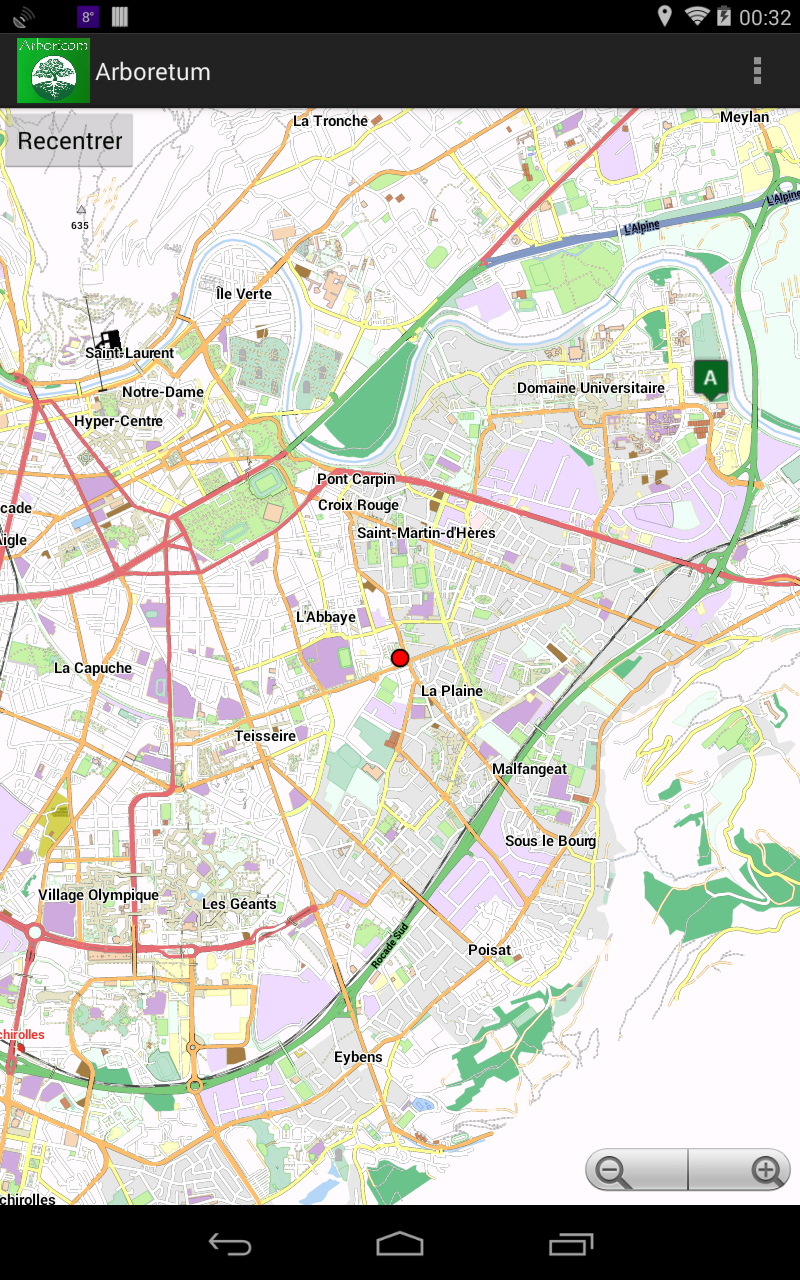
\includegraphics[width=5cm,height=7cm]{grenoble.png}
      \caption{Carte de Grenoble avec les marqueurs de position de l'arboretum et de l'utilisateur}
     \end{center}
    \end{figure}
			Il a été choisi de représenter l'utilisateur par un point plutôt qu'une flèche, du fait que nous n'avons pas réussi à implémenter la direction de celle-ci en fonction de l'orientation de la personne.
     \begin{figure}[H]
     \begin{center}
      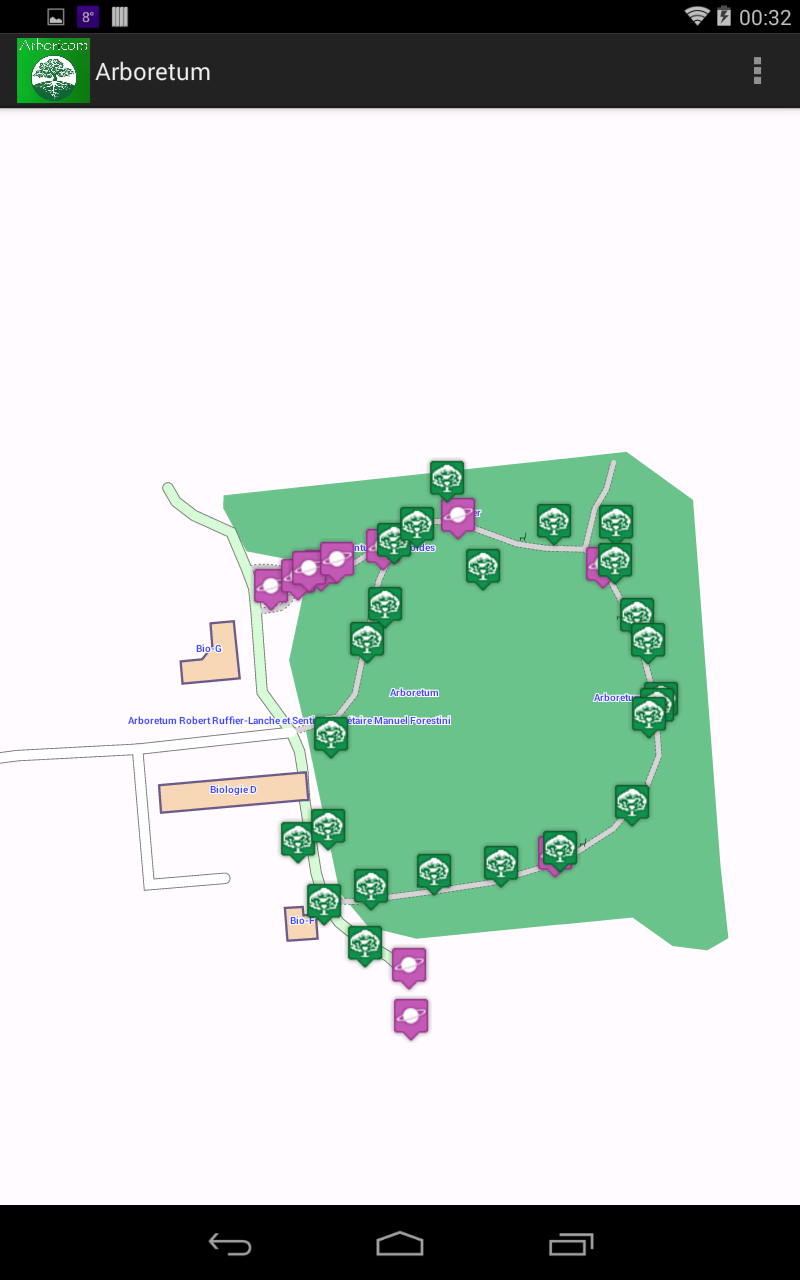
\includegraphics[width=7cm,height=10cm]{arbo.png}
      \caption{Carte de l'Arboretum avec ses différents points d'intérêts}
     \end{center}
    \end{figure}
			Pour les différents marqueurs des points d'intérêts, un clique sur ceux-ci entraine l'ouverture d'une boîte de dialogue. 
			Il a été décidé de passer celle-ci en noir, pour rendre son utilisation moins agressive à la vue. 
			
			\begin{figure}[H]
     \begin{center}
      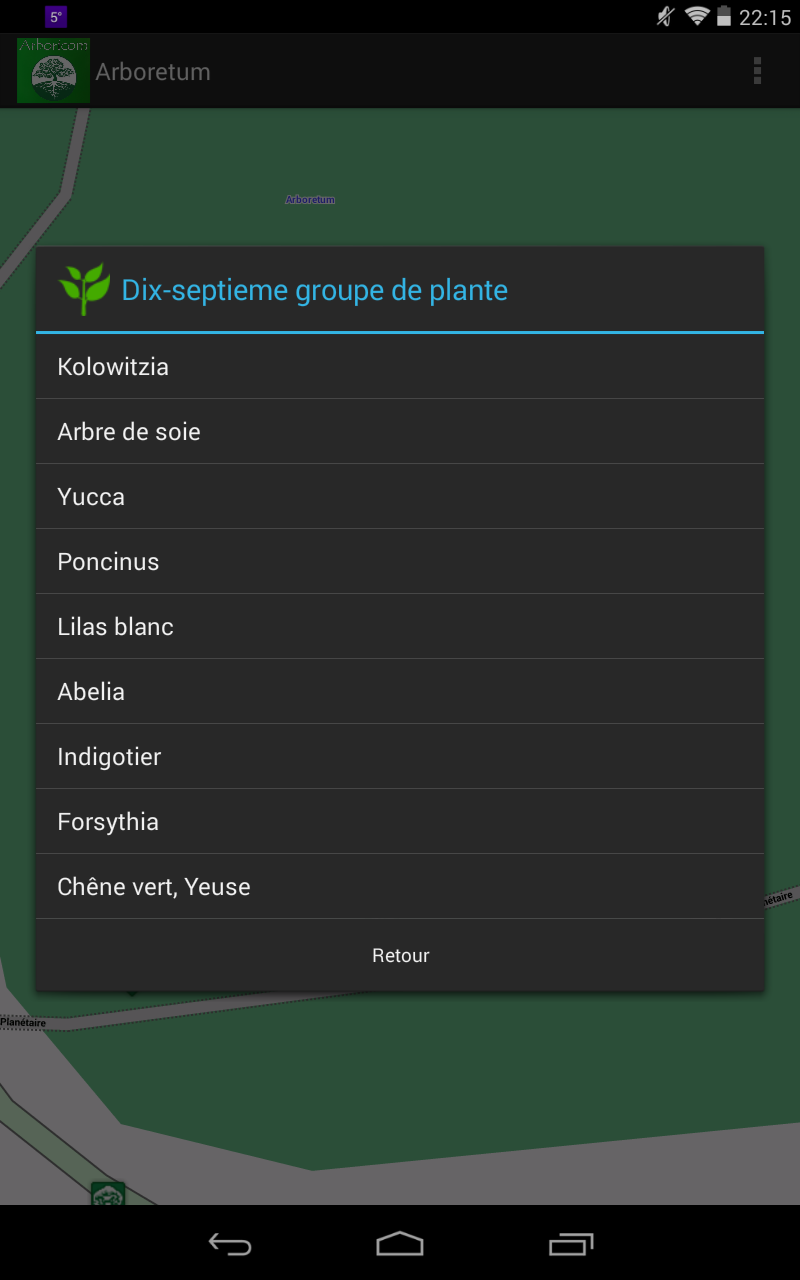
\includegraphics[width=5cm,height=7cm]{menuchoix.png}
      \caption{Exemple d'une boîte de dialogue pour le choix de la Webview}
     \end{center}
    \end{figure}
			Cette boîte de dialogue possède une icône représentant le type d'objet pour lequel la personne aurait besoin d'avoir plus d'informations. La personne peut au travers de cette boîte de dialogue choisir d'obtenir des informations supplémentaires sur le point d'intérêt.
		
		Pour le bon fonctionnement des cartes avec l’affichage de la position de l'utilisateur, le GPS est l'une des composantes principales de notre application. Le GPS est utilisé à deux moments précis. Lors de la visite en ligne de l'Arboretum, et pour se rendre à celui-ci. Le GPS est complété par les services de localisation. Ils ne sont activés que lorsque leur utilisation est nécessaire. Ils sont également désactivés lors de la mise en veille de l'écran par appel de la méthode onPause(), et remis en état de marche par OnResume(). Ses services sont utilisés pour représenter la personne sur une carte.
		
		Lors d'un passage proche d'un point d'intérêt, lors de la visite de l'arboretum en mode en ligne, un son de notification est joué si le son est activé. La détection se fait dans un carré de 3 mètres de côté centré sur le point en question. Deux sons différents sont disponibles, un pour les planètes, l'autre pour les plantes. Un problème dans l'application est à noter. La réactivation du son lors du passage proche d'un point d'intérêt entrainera un crash de l'application, par une erreur de mise en buffer du son.
		
		Une particularité importante d'android à connaître réside dans le système de rotation de l'écran. Une rotation entraine l'utilisation de la méthode onDestroy(), et donc de la méthode onCreate(), réinitialisant l'activité. Nous avons donc décidé de bloquer la rotation de l'écran pour pallier à ce problème. Une autre solution aurait été d'utiliser des méthodes d'android permettant de sauvegarder différentes variables afin de les restaurer, mais plus compliquer à mettre en place et non important selon nous.
		
		 \begin{figure}[H]
     \begin{center}
      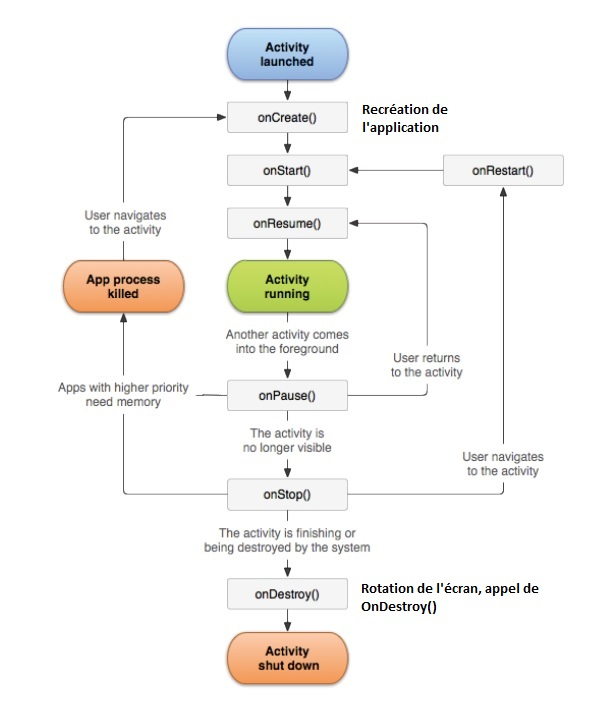
\includegraphics[width=11cm,height=10cm]{cyclerotation.jpg}
      \caption{Cycles de vie d'une application android}
     \end{center}
    \end{figure}
		
		\section{La gestion des Webviews et du Text-to-Speech}
		Les webviews utilisées dans notre application permettent d'afficher le contenu concernant les plantes/arbres et planètes. À chaque fois qu'un utilisateur clique sur un point d'intérêt, la webview correspondante est affichée à l'écran et est chargée dans une \emph{activity} dédiée. Cela permet de revenir à la carte. Sans cela, les webviews seraient chargées dans la même activity que la carte, et lorsque l'utilisateur appuierait sur le bouton \emph{retour}, il ne reviendrait pas à la carte, mais au menu de choix.
		
		De plus, le étant autorisé dans les webviews, un bouton est implémenté dans chacune des pages web. Cela permet d'appeler une fonction JavaScript qui va à son tour appeler une fonction java. Cette dernière permet de lancer le \emph{Text to speech} qui énoncera un texte.
		Le \emph{Text to speech} est chargé au démarrage de l’application et est initialisé au lancement de la webview. La classe \emph{WebAppInterface} sert d'interface pour utiliser la fonction java \emph{Speakout} qui permet l'énonciation du texte. Lorsqu'un utilisateur quitte la webview, le TTS est arrêté (même s'il est en train d'être utilisé). Cela libère de la mémoire RAM.
		
		Il y a cependant des limitations :
		\begin{itemize}
		\item Le texte est limité à 450 caractères en une seule fois
		\item Un nombre écrit avec des chiffres est converti en caractères alphabétiques
		\item Quelques problèmes d'élocution et de prononciation du texte
		 
		\end{itemize}
    \newpage
    \section{Le NFC}
      \subsection{Lecture d’un tag}
      La lecture d’un tag nfc est effectuée par le service nfc. Lorsqu’il détecte un tag, il envoie un des 3 types d’intents à une des applications 
      filtrant ces intents. Ces 3 intents sont NDEF\_DISCOVERED, TECH\_DISCOVERED et TAG\_DISCOVERED. 
      Vous pouvez voir comment est choisi le type d’intent envoyé dans le schéma suivant.
    \begin{figure}[H]
     \begin{center}
      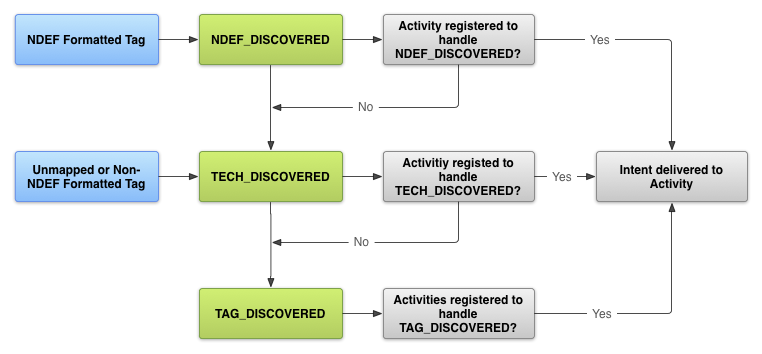
\includegraphics[width=15cm,height=7cm]{nfc_tag_dispatch.png}
      \caption{Type d'intent}
     \end{center}
    \end{figure}
      Au final, nous n’avons pas à choisir quel type d’intent nous recevons, car nos intent sont réceptionnés en foreground comme expliqué ci-après.
      
      \subsection{Écriture d'un tag}
      Pour écrire des tags spécifiques à notre application, plusieurs solutions étaient possibles.
      Nous avons choisi la plus simple qui est d’écrire dans le tag un message d’un type mime propre à notre application \textit{application/com.ricm.arboretum}. 
      Notre application est conçue pour lire des tags portant uniquement de ce type-là.
      
      \subsection{L’application}
      L’idée initiale était d’avoir une activity gérant seuls les intents émis par les tags NFC. 
      Ce ne fut pas possible, car le service NFC ouvre l’activity dans sa task \textit{service nfc}, on perd alors toutes les possibilités de retour 
      dans l’application. 
      Nous n’avons pas trouvé comment modifier ce mode d’ouverture et préféré adapter l’application à une nouvelle solution.
      
      La seconde solution était d’intercepter tous les intents en foreground. 
      C'est-à-dire qu’il n’est plus nécessaire d’inscrire notre activity à l’aide d’intent filter mais qu’à la place, 
      si l’application est active au premier plan, elle interceptera les intents NFC (passant un filtre) directement. 
      Cela pose un problème, l’application doit être ouverte pour réagir aux tags. 
      Ce problème est en partie contourné en ouvrant l’application à l’aide d’AAR.
      
      \subsection{Android application records(AAR)}
      Nos tags étant prévus pour être en extérieur dans un lieu public, il arrivera que des appareils sans l’application tentent de lire nos tags. 
      Dans les tags a été ajouté un message AAR (android application records). 
      Si un appareil sans l’application tente de lire le tag, il sera redirigé sur la page Play store de l’application, 
      dans le cas où l’application est déjà installée, elle sera simplement ouverte.
    
		\section{L'avenir de l'application}
		
		Plusieurs tests ont pus être effectués afin de valider le bon fonctionnement de l'application. En premier lieu, l'application a été utilisé par différents utilisateurs non informaticiens et informaticiens afin de voir leur réaction par rapport à l'application.

		Nous avons ensuite testé l'application sur des personnes de sachant pas très bien utilisé les appareils de type android et elles ont trouvés notre application ainsi que nos webviews simple d'utilisation et claire.

		En ce qui concerne notre précision au niveau du GPS, nous avons effectué plusieurs tests en direct de l'arboretum afin de déterminer quelle précision nous correspondait le mieux pour le lancement des détections sonores. Nous avons commencé avec un carré autour de notre position de 4m de diamètre. Cela était en réalité beaucoup trop grand et causait des soucis de son multiple. C'est également lors du premier test grandeur nature que nous nous sommes rendu compte du problème de rotation de l'écran qui redémarrait l'activité. Suite à ce premier test, nous avons donc bloqué la rotation de l'écran en format portrait, puis nous avons ajusté la zone de détection à un carré d'un mètre de côté. D'autres tests ont par la suite eu lieu entre nous, afin de corriger cette zone, pour arriver à un carré de 3 mètres de côtés. Un autre facteur important des tests a été la résolution d'une question grandissante, comment afficher au mieux les plantes de l'arboretum, celui-ci comptant un très grand nombre d'espèces. Nous avons donc décidé de créer des groupes de plantes par zone, et de recenser en majorité les plantes bordant les allées. 
		
		Un autre facteur du choix de la zone de détection pour les notifications ainsi que pour le groupement des plantes vient des erreurs GPS sur la zone, en moyenne de 3 à 5 mètres, mais allant dans certaines zones jusqu'à 8 mètres, voir 12, ce qui est une marge d'erreur non négligeable. Enfin, ce dernier test nous a permis de vérifier le bon fonctionnement de l'activation, désactivation du son. Le test a mis en évidence que l'activation du son lors de la visite ``en ligne'' de l'arboretum conduisait à un arrêt de l'application, si la personne se retrouve dans une zone de détection pour notification.
		
		La dernière série de tests a servi à l'implémentation du Text-to-Speech (\emph{tts}) de façon optimale. Nous avons remarqué que le \emph{tts} en français limite la lecture à 450 caractères environ, une limite que nous n'avons pas encore réussi à franchir. Un autre souci du \emph{tts} provient de la prononciation parfois difficile pour certains mots. Par exemple, afin d'obtenir une bonne prononciation du mot Mars, nous somme obligé de l'écrire Marsse (nous jouons sur la phonétique française). Néanmoins, il s'est avéré que le \emph{tts} est une technologie efficace, à la synthèse vocale et l’élocution plus que correcte.
		
		Pourquoi notre application ne peut pas être mise en ligne sur Android Market : 
En ce qui concerne notre application, celle-ci est fonctionnelle, mais nous devons la présenter à des professionnelles en développement android afin de savoir si notre application ne consomme pas trop de batterie, vérifier les droits d'auteurs pour plusieurs images, etc. Il reste également la question de l'arrêt causé par une erreur lors de l'utilisation de l'application dans le cas de la réactivation du son lors de la visite ``en ligne''.

De plus, nous devrions passer une semaine avec un spécialiste des plantes et/ou du directeur de l'arboretum afin de finaliser, changer, argumenter nos descriptions de nos plantes et planètes, et rajouter celles qui manquent à l'appel.

Nous pourrions ensuite mettre notre application aux mains d'une autre équipe qui pourraient l’intégrer dans une application de plus vaste envergure à savoir une visite guidée de Grenoble par exemple. Nous pourrions également prendre une main la gestion de cette application et nous en occuper personnellement.
		
		Un dernier problème qui pourrait être pointé du doigt est un souci d'affichage des \emph{Webviews}. Pour le moment, celles-ci se s'adaptent pas aux différents dispositifs, par exemple sur les tablettes Nexus 7, aucun problème n'est à noté, en revanche un Galaxy S3 ou un Xperia U fournissent des affichages moins agréables à la lecture.
		
    \section{Crédits}
		
    Cette application Android a été réalisée par une équipe d'étudiants en Réseaux Informatiques et Communication Informatique composée par 
    M. Jérôme BARBIER,Radhoane BENYOUNES, William BOBO, Rodolphe FREBY, Paul LABAT, supervisé par M. Augustin HUSSON et sous la tutelle 
    de M. Jacques LEMORDANT.

    \section{Remerciements}
    À Dana Fréby:
    \begin{itemize}
     \item Pour avoir effectué les relevés GPS nécessaires au positionnement des points d'intérêts du parc.
     \item Pour avoir testé le GPS par temps couvert et dégagé. 
     \item Pour avoir testé le son de l'application
    \end{itemize}
    
  À Didier Donzet, pour nous avoir gracieusement donné des tags NFC.
\end{document}